This section describes the computational realization of the local-geometry-aware contact model. The computational structure is organized around four aspects: discrete representation of local geometric fields on sparse narrow-band SDFs, coordinate transformation and packaging of patch-level geometric quantities, hierarchical acceleration for candidate-sample enumeration, and interface-level write-back of geometric feedforward into the complementarity solution chain. Overall, the realization follows the same principle as the methodology section: local geometric information only modifies the contact-constraint input and does not alter the dynamical structure of the underlying LCP module.

\subsection{Discrete representation of local geometric fields on sparse narrow-band SDFs}
The implementation uses the trilinear interpolation query interface provided by NanoVDB \cite{museth2021nanovdb} and employs a sparse narrow-band SDF (SNB-SDF) built around the geometric boundary as the underlying implicit representation. As shown in Fig. \ref{fig:snb_sdf}, only active voxels within the narrow band $|d|\le\tau$ are retained, while voxels far from the interface are pruned. This avoids the $\mathcal{O}(N^3)$ storage cost of dense voxel grids and focuses the queries of $\Phi$, $\nabla\Phi$, and local second-order geometric quantities on the neighborhoods that actually matter for contact.

\begin{figure}[htbp]
    \centering
    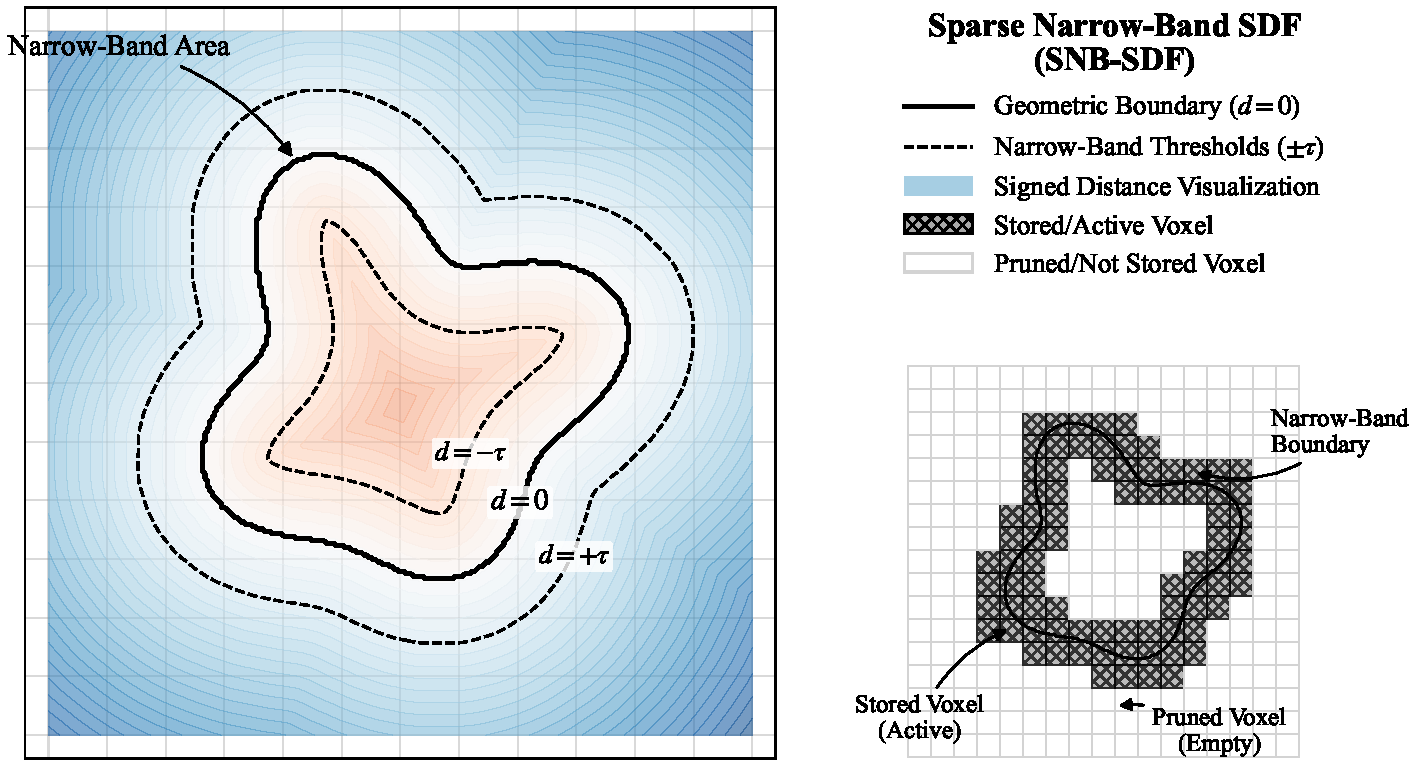
\includegraphics[width=0.98\linewidth]{SNB_SDF_Diagram_Compact_V2.pdf}
    \caption{Sparse narrow-band SDF (SNB-SDF). The left panel illustrates the continuous signed distance field, the geometric boundary $d=0$, and the narrow-band threshold $\pm\tau$; the lower-right panel illustrates the discrete voxel storage scheme, in which only voxels inside the narrow band are retained as active voxels while voxels far from the boundary are pruned}
    \label{fig:snb_sdf}
\end{figure}

Because discrete distance fields exhibit high-order discontinuities near voxel boundaries, the implementation does not compute the Hessian of the scalar distance field $\Phi$ directly. Instead, it first queries the unit normal field
\begin{equation}
    \mathbf{n} = \frac{\nabla \Phi}{\|\nabla \Phi\|},
\end{equation}
and then constructs the curvature tensor through central differencing:
\begin{equation}
    \mathbf{W} \approx \nabla \mathbf{n}.
\end{equation}
The differencing step size is chosen as
\begin{equation}
    h = 2 \cdot \text{voxel\_size}.
\end{equation}
The resulting $\mathbf{W}$ therefore corresponds to an approximation of the Weingarten map on the discrete SDF normal manifold.

\subsection{Coordinate mapping of local geometric quantities and patch encapsulation}
For each active contact sample, $\Phi$, the unit normal, and the curvature tensor $\mathbf{W}_M$ are first queried in model coordinates and then mapped into world coordinates through the rigid-body orientation matrix:
\begin{equation}
    \mathbf{W}_W = \mathbf{R}_{WM}\mathbf{W}_M\mathbf{R}_{WM}^T.
\end{equation}

During active-set construction, candidate samples are first filtered through a separating-velocity cutoff based on predicted normal relative velocity, so as to remove samples that are already clearly separating in the normal direction. The remaining candidates are then clustered into local patches according to spatial-radius and normal-angle thresholds. Patch normals are averaged and renormalized, whereas principal geometric quantities such as penetration depth $\Phi$, gradient, and Hessian are retained from the deepest sample. After this procedure, each patch is encapsulated as a local geometric proxy that can be inserted directly into contact-constraint assembly.

\subsection{Hierarchical candidate enumeration with OBB/BVH}
To reduce the query cost caused by dense surface sampling of follower bodies in continuous-sliding benchmarks, the implementation further introduces a static OBB/BVH broad phase on the sample side. This hierarchy is built in the follower's local coordinate frame. Each node stores a local OBB, a representative sample point, and the associated bounding radius. During simulation, it suffices to transform the representative point to world coordinates through the rigid-body pose and then into the model frame of the driving body's SDF for a lightweight $\Phi$ query.

Node-level pruning follows a conservative principle. A bounding-sphere lower bound of the driving geometry is first used to filter nodes that are clearly unable to contact. This is followed by conservative SDF pruning based on the representative point's $\Phi$ value, the node bounding radius, and a one-step motion margin. Only samples in unpruned leaf nodes proceed to accurate $(\Phi,\nabla\Phi)$ and, when needed, Hessian queries. The OBB/BVH layer therefore modifies only the candidate-enumeration strategy and does not alter leaf-level contact-sample construction, patch clustering, or the curvature-feedforward formula, which means that the final contact result is preserved.

This broad phase is enabled by default for the \texttt{SlidingPatch} path in continuous-sliding benchmarks such as the industrial cam, the eccentric disk--roller benchmark, and the Onset Stress Benchmark. For \texttt{CompactDiscrete} cases such as Twin Gear, where strong temporal coherence of local scanning is already present and contact switching is more compact, it is disabled by default and used only as an optional offline acceleration.

\subsection{Write-back of geometric feedforward into the right-hand side}
For each active patch, the implementation computes the second-order curvature compensation from the current-step relative contact-point velocity $\mathbf{v}_{rel}$:
\begin{equation}
    C_{curve} = \frac{1}{2} (\Delta t)^2 (\mathbf{v}_{rel})^T \mathbf{W}_{W} \mathbf{v}_{rel},
\end{equation}
and constructs the corrected effective contact gap
\begin{equation}
    \Phi_{eff} = \Phi + C_{curve}.
\end{equation}

The resulting $\Phi_{eff}$ is then written back into the contact-constraint interface and enters the underlying complementarity module as part of the right-hand side of the LCP equations. In this way, the computational realization preserves the parasitic right-hand-side injection structure introduced in the methodology: rather than altering the complementarity solution chain itself, it modifies the contact-constraint input through local geometric feedforward.

Algorithms \ref{alg:slidingpatch} and \ref{alg:compactdiscrete} summarize the computational paths of the two local contact representations. They share the same underlying LCP chain but differ fundamentally in candidate-sample screening, patch-level geometric encapsulation, and the conditions under which curvature terms are enabled.

\begin{algorithm}[htbp]
\caption{\texttt{SlidingPatch} pipeline for smooth continuous contact}
\label{alg:slidingpatch}
\begin{algorithmic}[1]
\Require Sample set $\mathcal{S}$, previous manifold $\mathcal{M}^{-}$, SDF interface
\Statex \textbf{Mode:} \texttt{SdfFirstOrder} or \texttt{SdfSecondOrder}
\Ensure Active contact patches with effective gaps $\Phi_{eff}$
\State Query $(\Phi,\nabla \Phi)$ for each sample in $\mathcal{S}$
\State Discard candidates failing the separating-velocity cutoff
\State Cluster the remaining candidates into local patches
\State Match current patches with $\mathcal{M}^{-}$ to preserve persistent-manifold identity
\State Update representative points through representative queries and local geometric fitting
\State Reject prematurely activated candidates that fail onset-aware filtering
\If{the current mode is \texttt{SdfSecondOrder}}
    \State Query the Hessian / Weingarten tensor at the representative geometry
    \State Compute $C_{curve} \gets \frac{1}{2}(\Delta t)^2 \mathbf{v}_{rel}^{T}\mathbf{W}\mathbf{v}_{rel}$
    \State Set $\Phi_{eff} \gets \Phi + C_{curve}$
\Else
    \State Set $\Phi_{eff} \gets \Phi$
\EndIf
\State Write the active patches into the LCP contact container
\end{algorithmic}
\end{algorithm}

\begin{algorithm}[htbp]
\caption{\texttt{CompactDiscrete} pipeline for compact or singular contact}
\label{alg:compactdiscrete}
\begin{algorithmic}[1]
\Require Sample set $\mathcal{S}$, SDF interface
\Statex \textbf{Mode:} \texttt{SdfFirstOrder} or \texttt{SdfSecondOrder}
\Ensure Compact active patch set retaining dominant geometry
\State Query $(\Phi,\nabla \Phi)$ for each sample in $\mathcal{S}$
\State Discard candidates failing the separating-velocity cutoff
\State Cluster the remaining candidates using spatial-radius and normal-angle thresholds
\State Average normals within each patch
\State Retain dominant/deepest geometry for $\Phi$, gradient, and Hessian
\State Truncate the active set according to the preset compact-patch budget
\If{the current mode is \texttt{SdfSecondOrder}}
    \State Compute local $C_{curve}$ on the retained patch geometry
    \State Set $\Phi_{eff} \gets \Phi + C_{curve}$
\Else
    \State Set $\Phi_{eff} \gets \Phi$
\EndIf
\State Write the compact active patches into the LCP contact container
\end{algorithmic}
\end{algorithm}
